\documentclass[11pt]{report}
\usepackage{graphicx}
\usepackage{tabularx}
\usepackage{graphicx}
\usepackage[margin=0.5in]{geometry}
\usepackage{listings,xcolor}
\lstset{
    string=[s]{"}{"},
    stringstyle=\color{blue},
    comment=[l]{:},
    commentstyle=\color{black},
    breaklines=true,
}
\PassOptionsToPackage{hyphens}{url}\usepackage{hyperref}
\begin{document}

\title{Assignment 3}
\author{Joshua Graham}

\maketitle
\pagebreak
\begin{abstract}
All Scripts used in the assignment can be found in the A4 folder, if needed.

\end{abstract}
\section{Problem 1}
	Question 1 was more a .txt file manipulation question than interacting with the outside world. The hardest part was getting the marks on the graph correct with R. I used the script scores.py to simplify the list from a key,value setup to just a single list of numbers sorted by value. This same script also prints out the values for mean, median, and standard deviation. I placed the markers for this manually, as well as the text that labels each listed value.
	
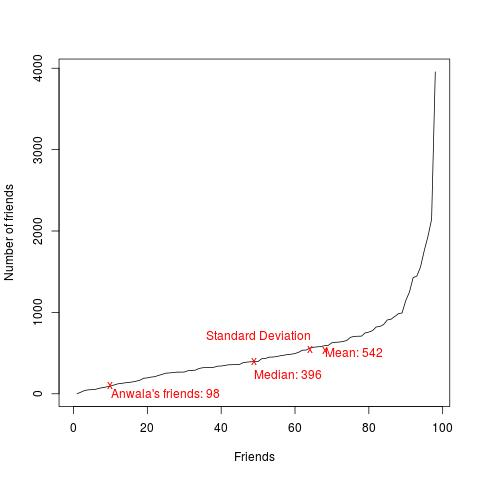
\includegraphics[scale=1]{A1.jpeg}
\pagebreak
\section{Question 2}
	Question 2 was harder, but it was all information we'd worked with before. I setup the script twt.py to generate a file that matches the format of question 1's acnwala-friendscount.csv. This was done so I could use the same script to geneate output for this question. It was here that I made the python script use a function instead of hard coding all the values in, this made automation easier. 
	
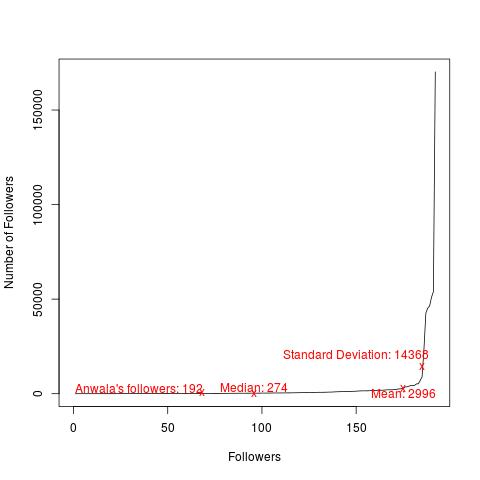
\includegraphics[scale=1]{A2.jpeg}

\end{document}